% -*- TeX-command-extra-options: "-shell-escape"; TeX-engine: xetex; -*-
\documentclass{beamer}

\usetheme[numbering=none]{m}
\usepackage{fontspec}
\usepackage[ngerman]{babel}
\usepackage{standalone}
\usepackage{tikz}
\usepackage{tikz-qtree}
\usepackage{amsmath}
\usepackage{minted}

\usetikzlibrary{fit, calc, decorations, decorations.pathreplacing, shapes,
  matrix, positioning}

\tikzset{onslide/.code args={<#1>#2}{%
  \only<#1>{\pgfkeysalso{#2}} % \pgfkeysalso doesn't change the path
}}

\tikzset{temporal/.code args={<#1>#2#3#4}{%
  \temporal<#1>{\pgfkeysalso{#2}}{\pgfkeysalso{#3}}{\pgfkeysalso{#4}}%
}}

\tikzset{
  every tree node/.style = {align=center, inner sep=5pt, text centered, font=\sffamily, rectangle, black, draw=black, very thick},
  every leaf node/.style = {draw=none},
  n/.style = {draw=none},
  hidden/.style = {opacity=0},
  uncover/.style = {temporal=#1{hidden}{}{}},
  level distance=1.5cm,sibling distance=0.5cm
}

\renewcommand{\UrlFont}{\scriptsize}

\begin{document}
\title{Verifizierte Implementierung einer Mapping-Datenbank in Coq}
\subtitle{wissenschafliches Forum 2015}
\author{Benno Fünfstück}
\date{\today}
\institute{
  \begin{tabbing}
    Betreuer: \=Dr. Hendrik Tews \& Dr. Thomas Türk\\
              \>FireEye Technologie Deutschland GmbH
  \end{tabbing}
}

\maketitle

\begin{frame}{Gliederung}
  \setbeamertemplate{section in toc}[sections numbered]
  \tableofcontents
\end{frame}

\section{Microkern und Mapping-Datenbank}

\begin{frame}{Entwicklung des Linux-Kerns}
  \centering
  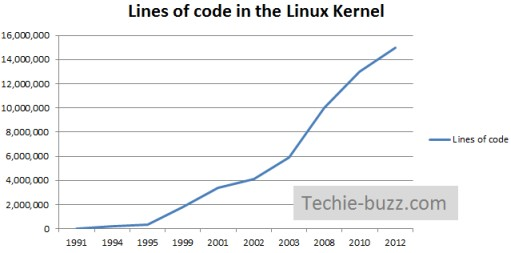
\includegraphics[width=\textwidth]{img/linux-loc2.jpg}\\
  \vfill
  \scriptsize{Quelle:} \url{http://cache.techie-buzz.com/images4/chinmoy/linux-kernel-rise.jpg}
\end{frame}

\begin{frame}{Lösungsansatz: Microkern}
  \begin{itemize}
    \item Nur wesentliche Funktionen im Kern
    \item NOVA-Microkern: ca. 10000 Zeilen Quelltext
    \item weniger Fehler im Kern
  \end{itemize}
\end{frame}

\begin{frame}{Capabilities}
  \documentclass{standalone}

\usepackage{tikz}

\usetikzlibrary{fit, calc, decorations, decorations.pathreplacing}

\begin{document}
  \begin{tikzpicture}[
    x=1mm, 
    y=1mm,
    selektor/.style={
      fill=blue!5!white, 
      text=blue!80!black,
      draw=blue!80!black,
      circle
    },
    task/.style={draw=green!60!black, text=green!60!black, rectangle},
    mempage/.style={draw, rectangle, minimum width=1cm, inner sep=0, minimum height=1cm}]
   \path
     node(pd11) at (  0, 0)  [selektor] {1}
     node(pd12) at ( 10,10)  [selektor] {2}
     node(pd13) at ( 20, 0)  [selektor] {3}
     node(pd21) at ( 75, 0)  [selektor] {1}
     node(pd22) at ( 87,10)  [selektor] {2}
     node(pd23) at (100, 0)  [selektor] {3};

   \node[task, label={[green!60!black]Prozess 1}, fit=(pd11) (pd12) (pd13)] {};
   \node[task, label={[green!60!black]Prozess 2}, fit=(pd21) (pd22) (pd23)] {};

   \foreach \x[count=\i] in {0,10,...,90}
     \node[mempage, at={(\x, -20)}](mem\i) {\i}; 
   \node[mempage, at={(100,-20)}](memlast){\dots};

   \begin{scope}[very thick]
     \draw[->] (pd11) -- (mem1.north);
     \draw[->] (pd12) -- (mem3.north);
     \draw[->] (pd13) .. controls (40,0) .. ($(mem6.north west)!.35!(mem6.north east)$);
     \draw[->] (pd21) .. controls (60,0) .. ($(mem6.north west)!.55!(mem6.north east)$);
     \draw[->] (pd22) -- ($(mem9.north west)!.35!(mem9.north east)$);
     \draw[->] (pd23) -- ($(mem9.north west)!.55!(mem9.north east)$);
   \end{scope}

   \draw[decorate, decoration={brace, amplitude=5}, thick]
     (memlast.south east) -- (mem1.south west);
   \node[at=($(memlast.south east)!.5!(mem1.south west)$), anchor=north, yshift=-5]
     {Speicher}; 
  \end{tikzpicture}
\end{document}

\end{frame}

\begin{frame}{Mapping-Datenbank}
  \centering
  \documentclass{standalone}

\usepackage{tikz}
\usetikzlibrary{fit, shapes}

\begin{document}
\begin{tikzpicture} [
  y=1mm,
  x=1mm,
  task/.style={draw=green!60!black, text=green!60!black, ellipse}
  ]
  \node(task1)[task, at={(0,0)}]{Prozess 1};
  \node(task2)[task, at={(30,0)}]{Prozess 2};
  \node(map-db)[task, at={(15,40)}]{Mapping-Datenbank};
  \node(kern)[rectangle, draw, at={(15,60)}]{Microkern};
  
  \draw[<->] (task1) -- (map-db);
  \draw[<->] (task2) -- (map-db);
  \draw[<->] (map-db) -- (kern);
\end{tikzpicture}
\end{document}
\end{frame}

\section{Implementierung}
\begin{frame}{Operationen der Mapping-Datenbank}
\begin{itemize}
  \item Eintrag anlegen
  \item Eintrag entfernen
  \item Zugriff auf ein bestimmtes Kernobjekt entziehen
\end{itemize}
\end{frame}

\begin{frame}{Datenstruktur der Mapping-Datenbank}
  \centering
  \documentclass{standalone}

\usepackage{tikz}

\usetikzlibrary{fit, calc, shapes, matrix}

\begin{document}
\begin{tikzpicture} [
  proc/.style={
    draw, circle, fill=green!15!white, text=green!60!black, draw=green!80!black
  },
  sel/.style={draw, circle, fill=blue!15!white, text=blue!80!black, draw=blue!80!black},
  ko/.style={
    draw, circle, fill=orange!15!white, text=orange!60!black, draw=orange!80!black},
  heading/.style={draw=none, fill=none, rectangle}
  ]
  \matrix[row sep=4mm, column sep=1.5cm] { 
    \node[proc, heading]{Prozess}; & \node[sel, heading]{Capability}; & \node[ko, heading]{Kernobjekt}; \\
    \node(p1)[proc]{3}; & \node(s11)[sel]{6}; & \node(k11)[ko]{A}; \\
                        & \node(s12)[sel]{7}; & \node(k12)[ko]{C}; \\
                        & \node(s13)[sel]{9}; & \node(k13)[ko]{B}; \\
    \node(p2)[proc]{7}; & \node(s21)[sel]{4}; & \node(k21)[ko]{D}; \\
                        & \node(s22)[sel]{8}; & \node(k22)[ko]{A}; \\
  };
  \node(s1)[fit=(s11) (s13) (k11) (k13), draw]{};
  \node(s2)[fit=(s21) (s22) (k21) (k22), draw]{};
  \begin{scope}[thick]
    \draw[->] (p1) -- (p1 -| s1.north west);
    \draw[->] (p2) -- (p2 -| s2.north west);
    \draw[->] (s11) -- (k11);
    \draw[->] (s12) -- (k12);
    \draw[->] (s13) -- (k13);
    \draw[->] (s21) -- (k21);
    \draw[->] (s22) -- (k22);
  \end{scope}
\end{tikzpicture}
\end{document}
\end{frame}

\begin{frame}{Darstellung der Zuordnung}
  \centering
  \begin{tabular}{|c|c|}
    \hline
    Capability & Kernobjekt \\ \hline
    2          & B \\           
    5          & E \\
    1          & A \\
    4          & D \\
    3          & C \\
    \dots      & \dots\\
    \hline
  \end{tabular}
\end{frame}

\begin{frame}{Binärer Baum}
  \centering
  \Tree [.$(2,B)$ [.$(1,A)$ ] \edge[onslide=<2->red];[.$(4,D)$ \edge[onslide=<3->red];[.$(3,C)$ ] [.$(5,E)$ ] ] ]
\end{frame}

\begin{frame}{Entartung}
  \begin{tikzpicture}
  \node<1->(n1){\Tree [.\node(r1){$1$}; ]};
  \node<2->(n2)[at={($(n1.north east) + (0.7cm,0)$)}, anchor=north west]{
    \Tree [.\node(r2){$1$}; \edge[n];{} [.2 ] ]
  };
  \node<3->(n3)[at={($(n2.north east) + (0.5cm,0)$)}, anchor=north west]{
    \Tree [.\node(r3){$1$}; \edge[n];{} [.2 \edge[n];{} [.3 ] ] ]
  };
  \node<4->(n4)[at={($(n3.north east) + (0.5cm,0)$)}, anchor=north west]{
    \Tree [.\node(r4){$1$}; \edge[n];{} [.2 \edge[n];{} [.3 \edge[n];{} [.4 ] ] ] ]
  };
  \draw<2->[->, ultra thick] (0.75,0) -- (1.4,0);    
  \draw<3->[->, ultra thick] (2.9,0) -- (3.9,0);    
  \draw<4->[->, ultra thick] (5.4,0) -- (7.0,0);    
  \end{tikzpicture}
\end{frame}

\begin{frame}{Rotation}
  \documentclass{standalone}

\usepackage{tikz}
\usepackage{tikz-qtree}

\usetikzlibrary{fit, calc, shapes, positioning}

\begin{document}
\begin{tikzpicture}
  [every tree node/.style = {
    align=center, inner sep=2pt, text centered, font=\sffamily, 
    rectangle, black, draw=black, very thick},
   every leaf node/.style = {draw=none},
   n/.style = {draw=none},
   level distance=0.75cm, sibling distance=0.5cm,
   subtree/.style = 
     {isosceles triangle, shape border rotate=90, anchor=north, yshift=1mm, inner sep=0cm}
  ]
  \node(before) {
    \Tree [.\node[color=red]{A}; 
      [.\node[color=green!80!black]{B}; 
        [.\node[subtree, minimum height=1.75cm]{C}; ]
        [.\node[subtree, minimum height=1cm]{D}; ]        
      ]
      [.\node[subtree, minimum height=1cm]{E}; ] ]
  }; 
  \node(after) [at={($(before.east) + (1.5cm,0)$)}, anchor=west] {
    \Tree [.\node[color=green!80!black]{B}; 
      [.\node[subtree, minimum height=1.75cm]{C}; ] 
      [.\node[color=red]{A}; 
        [.\node[subtree, minimum height=1cm]{D}; ] 
        [.\node[subtree, minimum height=1cm]{E}; ] ] ]
  };
  \draw[->, ultra thick] ($(before.east) + (0.5cm,0)$) -- ($(after.west) - (0.5,0)$); 
\end{tikzpicture}
\end{document}
\end{frame}

\begin{frame}{Rotation: Beispiel}
  \centering
  \begin{tikzpicture}
    \Tree 
      [.\node[onslide=<3->{red}]{5};
        [.\node[onslide=<3->{color=green!80!black}]{3}; [.2 
          \edge[temporal=<2>{n}{red}{}];\node[every tree node, uncover=<2->, onslide=<2>{red}]{1}; ] 
          [.4 ] ]
        [.6 ]
      ];
    \begin{scope}[xshift=5cm, uncover=<4->]
      \Tree
        [.\node[color=green!80!black]{3};
          [.2 [.1 ] ]
          [.\node[color=red]{5}; [.4 ] [.6 ] ]
        ];
    \end{scope}
    \draw<4->[->, very thick] (2.0,-1) -- (3.2,-1);
  \end{tikzpicture}
\end{frame}

\begin{frame}{Vergleich mit Listenimplementierung}
 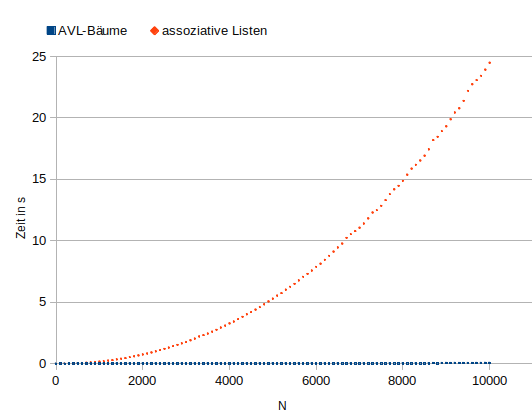
\includegraphics[height=0.8\textheight, width=\textwidth]{../paper/bench.png}
\end{frame}

\section{Verifikation}
\begin{frame}{Möglichkeiten zur Überprüfung}
  \begin{itemize}
    \item Manuelles Testen $\implies$ aufwändig, wenig Fälle abdeckbar
    \item Automatisiertes Testen $\implies$ weniger aufwändig, aber immer noch
      nicht alle Fälle testbar
    \item Verifikation $\implies$ Beweis, gilt für alle Fälle
    \item Coq ist ein interaktiver Theorembeweiser $\implies$ Beweise werden
      durch den Computer überprüft.
  \end{itemize}
\end{frame}

\begin{frame}{Bewiesene Eigenschaften}
  \begin{enumerate}
    \item Die angestrebte Veränderung wird durchgeführt
    \item Es finden keine weiteren Veränderungen statt
    \item Alle Invarianten werden beibehalten 
  \end{enumerate}
  $\implies$ nur die angestrebte Veränderung wird durchgeführt.
\end{frame}

\begin{frame}[fragile]{Beispiel: Anlegen eines Mappings}
  \begin{minted}[fontsize=\scriptsize]{coq}
Theorem create_has_mapping :
 forall (db:mapping_db) (pd:N) (sel:N) (ko:kernel_object),
  mapping_db_inv db -> 
  has_mapping pd sel ko (create_mapping pd sel ko db).
  \end{minted}
\end{frame}

\begin{frame}[fragile]{Beispiel: Anlegen eines Mappings}
  \begin{minted}[fontsize=\scriptsize]{coq}
Theorem create_preserve_other :
 forall (db:mapping_db) (pd pd':N) (sel sel':N) 
        (ko ko':kernel_object),
  (pd' <> pd \/ sel' <> sel) -> mapping_db_inv db ->
  (has_mapping pd sel ko db
   <-> has_mapping pd sel ko (create_mapping pd' sel' ko' db)).
  \end{minted}
\end{frame}

\begin{frame}[fragile]{Beispiel: Anlegen eines Mappings}
  \begin{minted}[fontsize=\scriptsize]{coq}
Theorem create_invariant :
 forall (db:mapping_db) (pd:N) (sel:N) (ko:kernel_object),
  mapping_db_inv db ->
  mapping_db_inv (create_mapping pd sel ko db).
  \end{minted}
\end{frame}

\section{Ergebnisse und Ausblick}

\begin{frame}{Ergebnisse}
  \begin{itemize}
    \item 2000 Zeilen Quelltext
    \item verifizierte Implementierung von AVL-Bäumen in Coq
    \item abstrakte Implementierung und Verifikation einer Mapping-Datenbank
    \item durch Verifikation wurden mehrere Fehler gefunden 
      \begin{itemize}
        \item Fehler bei der Implementierung des Löschens
        \item Falsche Anpassung der Balance im Falle einer Rotation
      \end{itemize}
  \end{itemize}
\end{frame}

\begin{frame}{Ausblick}
  \begin{itemize}
    \item Verknüpfung mit Operationen des Microkerns
    \item Refinement auf C-Implementierung
  \end{itemize}
\end{frame}

\begin{frame}{Fragen?}
  \begin{itemize}
    \item Bildquellen
      \begin{itemize}
        \item \url{http://cache.techie-buzz.com/images4/chinmoy/linux-kernel-rise.jpg}
      \end{itemize}
    \item \large Vielen Dank für die Aufmerksamkeit!
  \end{itemize}
\end{frame}

\end{document}
